%\section{Introduction}
%


%%%%%%%%%%%%%%%%%%%%%%
%%%%%%%%%%%%%%%%%%%%%%
%%%%%%%%%%%%%%%%%%%%%%
\subsection{Research Problem}
\begin{frame}{Research Problem}
The integration between graph and ``semi-structured nested'' data requires a new data model and a common query language.
\begin{enumerate}
\item<1-> Graph and Semistructured data are \alert{orthogonal} data representations.
\item<2-> The outcome of the data integration process should be represented into one \alert{general data model}.
\item<3-> Current query languages do not support most of the tasks required by \alert{data integration}.
\end{enumerate}

\note<1->{Oggi giorno sono disponibili sempre pi\`u dati a grafo e semistrutturati.\\
	\medskip
	
	Mentre i dati annidati semistrutturati vengono utilizzati nei DW per effettuare aggregazioni ed astrazioni sui dati originali, i dati a grafo rappresentano meglio relazioni tra entit\`a.}
\end{frame}

\begin{lucido}[Data Integration: Background]
	\smartdiagramset{sequence item font size=\footnotesize}
	\smartdiagram[sequence diagram]{
		Translation,
		Schema Alignment,
		\alert{Resolution},
		\alert{Sources}}
	\begin{enumerate}
		\item Translating the sources to the most general representation.
		\item Aligning local schemas to hub schemas.
		\item \alert{Solving the alignments over the data}.
		\item \alert{Integrate the solved sources}.
	\end{enumerate}
\note{Prima di risolvere algoritmicamente il più problema più generale di effettuare operazioni più simili alle graph grammars con pattern matching e rescritture (ovvero, ``rewriting''), ci focalizziamo su un sottoproblema specifico, che è quello della creazione di grafi annidati a partire dai grafi dati inizialmente.}
\end{lucido}

%%%%%%%%%%%%%%%%%%%%%%
%%%%%%%%%%%%%%%%%%%%%%
%%%%%%%%%%%%%%%%%%%%%%
\subsection{Research Questions}
\begin{frame}{Research Questions}
\begin{enumerate}[<+->]
\item[\refstepcounter{enumi}\textbf{\alert{\arabic{enumi}.}}] Is it possible to define a binary graph operator allowing graph combinations? \textbf{Graph Joins}. Is it possible to perform it efficiently? \textbf{GCEA (and GCLA) Algorithm}.

\item[\refstepcounter{enumi}\textbf{\alert{\arabic{enumi}.}}] Is it possible to represent graphs allowing arbitrary nestings? \textbf{Nested Graphs}.

\item[\refstepcounter{enumi}\textbf{\alert{\arabic{enumi}.}}] Is it possible to arbitrarily nest one single graph via one single operator, generalizing summarization and allowing graph matching and rewriting?
\textbf{Graph Nesting \& THoSP}
\item {\footnotesize Is it possible to define a generalize semistructured model allowing the representation of most of the very well known data models?
\textsc{Generalized Semistructured (data) Model}}.


\item {\footnotesize Is it possible to define one query language allowing  queries in all the (semi)structured data representations and to provide data integration tasks over the Generalized Semistructured Model?
\textsc{Generalized Semistructured Query Language}}
\end{enumerate}

\end{frame}




%\section{Graph Joins}
%%%%%%%%%%%%%%%%%%%%%%%
%%%%%%%%%%%%%%%%%%%%%%
%%%%%%%%%%%%%%%%%%%%%%

\begin{lucido}[Research Problem]
	\begin{enumerate}
		\setbeamertemplate{enumerate items}[square]
		\item  Despite the term ``join'' appearing in the graph database literature, such operator cannot be used to combine two distinct graphs, as for table joins in the relational model. They currently require to combine two operations, which combination results into an inefficient query plan:
		\begin{itemize}
			\item \alert{path joins} (currently simply called ``joins''), for graph traversals.
			\item \alert{construct} to create a graph from the matched paths.
		\end{itemize}
		\item Graph Joins are not Relations Joins, but ``Graph Products''.
	\end{enumerate}
\end{lucido}


%%%%%%%%%%%%%%%%%%%%%%
%%%%%%%%%%%%%%%%%%%%%%
%%%%%%%%%%%%%%%%%%%%%%
\begin{lucido}[Research Goals]
	\begin{enumerate}[<+->]
		\setbeamertemplate{enumerate items}[circle]
		\item The physical model must allow a quick access to the data structures, reduce the number of join operations and allow a quick serialization of both operand and index results.
		\item The join definition over the logical data model must be flexible enough to support further extensions (modularity, compositionality and properties preserving).
	\end{enumerate}
\end{lucido}
%%%%%%%%%%%%%%%%%%%%%%%
%%%%%%%%%%%%%%%%%%%%%%
%%%%%%%%%%%%%%%%%%%%%%
\begin{lucido}[Example (Conjunctive EquiJoin)]
	This is an example of a possible graph join query:


\begin{tcolorbox}[title=A Graph Join Query]
		Consider an on-line service such as \yellowemph{ResearchGate}
		where researchers can \textup{follow} each others' work, and a \yellowemph{citation graph}.
		\yellowemph{Return the paper graph} where \remark{a paper cites another one iff. the \greenemph{first
				author  of the first paper \textit{follows} the first author of} \greenemph{the second}}.
	\end{tcolorbox}
	
	\begin{itemize}
		\item \yellowemph{Binary operator returning just one graph}.
		\item \greenemph{Vertex conditions are ($\theta$-)join conditions}.
		\item \remark{A way to combine the edges is determined}.
	\end{itemize}
\end{lucido}

%%%%%%%%%%%%%%%%%%%%%%
%%%%%%%%%%%%%%%%%%%%%%
%%%%%%%%%%%%%%%%%%%%%%
\begin{lucido}[Operands in Property Graph Data Model]
	\begin{tikzpicture}
\clip (0.3,-2.5) rectangle (7.7, 1);
\node[user] (a1) at (2,.25) {\user{Alice}{$t_1$}};
\node[user] (a3) at (2,-2.25) {\user{Carl}{$t_1$}};
\node[user] (a2) at (6.3,.25) {\user{Bob}{$t_2$}};
\node[user] (a4) at (6.3,-2.25) {\user{Dan}{$t_2$}};

\path[->,orange] (a1.north east) edge node [anchor=south,sloped] {\{Follows\}} (a2.north west);
\path[->,orange] (a2.south east) edge  node [anchor=south,sloped] {\{Follows\}\qquad} (a4.north east);
\path[<-,orange] (a3.north west) edge node [anchor=north,sloped] {\{Follows\}\qquad} (a1.south west);
\path[<-,orange] (a3.east) edge node [anchor=south,sloped] {\{Follows\}\qquad} (a4);
\end{tikzpicture}

	\begin{tikzpicture}
\clip (0.3,-3) rectangle (10.1, 1.7);
\node[proj] (a1) at (2,0) {\proj{Alice}{Graphs}};
\node[proj] (a1b) at (5,0) {\proj{Alice}{Join}};
\node[proj] (a3) at (5,-2) {\proj{Carl}{Projection}};
\node[proj] (a2) at (8.3,0) {\proj{Bob}{OWL}};
\node[proj] (a4) at (8.3,-2) {\proj{Dan}{$\mu$-calc}};

\path[->,purple] (a1.north east) edge [bend left=40] node [anchor=south,sloped] {\{Cites\}} (a2.north west);
\path[->,purple] (a2.south west) edge  node [anchor=south,sloped] {\{Cites\}\qquad} (a3.north east);
\path[<-,purple] (a3.north west) edge node [anchor=north,sloped] {\{Cites\}\qquad} (a1b.south west);
\path[->,purple] (a3.south) edge [bend right=30] node [anchor=south,sloped] {\{Cites\}} (a4.south);
\end{tikzpicture}
\end{lucido}

%%%%%%%%%%%%%%%%%%%%%%
%%%%%%%%%%%%%%%%%%%%%%
%%%%%%%%%%%%%%%%%%%%%%
\begin{lucido}[Conjunctive EquiJoin]
	\begin{tikzpicture}
	%% Operand Left
	\begin{scope}[scale=0.6,yshift=5.5cm,xshift=0cm,every node/.style={transform shape}]
	\node[user2] (a1) at (2,.25) {\user{Alice}{$t_1$}};
	\node[user2] (a3) at (2,-2.25) {\user{Carl}{$t_1$}};
	\node[user2] (a2) at (6.3,.25) {\user{Bob}{$t_2$}};
	\node[user2] (a4) at (6.3,-2.25) {\user{Dan}{$t_2$}};
	
	\path[->,orange] (a1.north east) edge node [anchor=south,sloped] {\{Follows\}} (a2.north west);
	\path[->,orange] (a2.south east) edge  node [anchor=south,sloped] {\{Follows\}\qquad} (a4.north east);
	\path[<-,orange] (a3.north west) edge node [anchor=north,sloped] {\{Follows\}\qquad} (a1.south west);
	\path[<-,orange] (a3.east) edge node [anchor=south,sloped] {\{Follows\}\qquad} (a4);
	
	\onslide<2>
	\node[user3] (a1) at (2,.25) {\user{Alice}{$t_1$}};
	\onslide<3>
	\node[user3] (a2) at (6.3,.25) {\user{Bob}{$t_2$}};
	\onslide<4>
	\node[user3] (a3) at (2,-2.25) {\user{Carl}{$t_1$}};
	\onslide<5>
	\node[user3] (a4) at (6.3,-2.25) {\user{Dan}{$t_2$}};
	\onslide<6>
	\path[->,orange,line width=1mm] (a1.north east) edge node [anchor=south,sloped] {\{Follows\}} (a2.north west);
	\path[<-,orange,line width=1mm] (a3.north west) edge node [anchor=north,sloped] {\{Follows\}\qquad} (a1.south west);
	\onslide<1->
	\end{scope}
	
	%% Operand Right
	\begin{scope}[scale=0.6,yshift=-4cm,xshift=0cm,every node/.style={transform shape}]
	\node[proj2] (a1) at (2,0) {\proj{Alice}{Graphs}};
	\node[proj2] (a1b) at (5,0) {\proj{Alice}{Join}};
	\node[proj2] (a3) at (5,-2) {\proj{Carl}{Projection}};
	\node[proj2] (a2) at (8.3,0) {\proj{Bob}{OWL}};
	\node[proj2] (a4) at (8.3,-2) {\proj{Dan}{$\mu$-calc}};
	
	\path[->,purple] (a1.north east) edge [bend left=40] node [anchor=south,sloped] {\{Cites\}} (a2.north west);
	\path[->,purple] (a2.south west) edge  node [anchor=south,sloped] {\{Cites\}\qquad} (a3.north east);
	\path[<-,purple] (a3.north west) edge node [anchor=north,sloped] {\{Cites\}\qquad} (a1b.south west);
	\path[->,purple] (a3.south) edge [bend right=30] node [anchor=south,sloped] {\{Cites\}} (a4.south);
	
	\onslide<2>
	\node[proj3] (a1) at (2,0) {\proj{Alice}{Graphs}};
	\node[proj3] (a1b) at (5,0) {\proj{Alice}{Join}};
	\onslide<3>
	\node[proj3] (a2) at (8.3,0) {\proj{Bob}{OWL}};
	\onslide<4>
	\node[proj3] (a3) at (5,-2) {\proj{Carl}{Projection}};
	\onslide<5>	
	\node[proj3] (a4) at (8.3,-2) {\proj{Dan}{$\mu$-calc}};
	\onslide<6>
	\path[->,purple,line width=1mm] (a1.north east) edge [bend left=40] node [anchor=south,sloped] {\{Cites\}} (a2.north west);
	\path[<-,purple,line width=1mm] (a3.north west) edge node [anchor=north,sloped] {\{Cites\}\qquad} (a1b.south west);
	\onslide<1->
	\end{scope}
	
	%% Result
	\begin{scope}[scale=0.6,yshift=2.8cm,xshift=12cm,every node/.style={transform shape}]		
	
	\onslide<2>
	\node[result2] (a1) at (1,0) {\result{Alice}{Graphs}};
	\node[result2] (a2) at (5.5,0) {\result{Alice}{Join}};
	\onslide<3>
	\node[result2] (a3) at (1,-7.4) {\result{Bob}{OWL}};
	\onslide<4>
	\node[result2] (a4) at (1,-3.7) {\result{Carl}{Projection}};
	\onslide<5>
	\node[result2] (a5) at (5.5,-7.4) {\result{Dan}{$\mu$-calc}};
	\onslide<3->
	\node[result] (a1) at (1,1) {\result{Alice}{Graphs}};
	\node[result] (a2) at (5.5,1) {\result{Alice}{Join}};
	\onslide<4->
	\node[result] (a3) at (1,-7.4) {\result{Bob}{OWL}};
	\onslide<5->
	\node[result] (a4) at (1,-3.7) {\result{Carl}{Projection}};
	\onslide<6->
	\node[result] (a5) at (5.5,-7.4) {\result{Dan}{$\mu$-calc}};
	\path[->,purple!60!orange,very thick,dotted] (a1.north west) edge [bend right=33] node [anchor=south,sloped] {\{Follows,Cites\}} (a3.north west);
	\path[->,purple!60!orange,very thick,dotted] (a2) edge  node [anchor=north,sloped] {\{Follows,Cites\}} (a4.north east);
	\end{scope}
	
	
	\node<2-5> at (3,0) {\textbf{1. Vertex Join}};
	\node<6-> at (3,0) {\textbf{2. Combining Edges}};
	
	\end{tikzpicture}
\end{lucido}


%%%%%%%%%%%%%%%%%%%%%%
%%%%%%%%%%%%%%%%%%%%%%
%%%%%%%%%%%%%%%%%%%%%%
\begin{lucido}[Disjunctive EquiJoin]
		\begin{tikzpicture}
%% Operand Left
\begin{scope}[scale=0.6,yshift=5.5cm,xshift=0cm,every node/.style={transform shape}]
\node[user2] (a1) at (2,.25) {\user{Alice}{$t_1$}};
\node[user2] (a3) at (2,-2.25) {\user{Carl}{$t_1$}};
\node[user2] (a2) at (6.3,.25) {\user{Bob}{$t_2$}};
\node[user2] (a4) at (6.3,-2.25) {\user{Dan}{$t_2$}};
\path[->,orange] (a1.north east) edge node [anchor=south,sloped] {\{Follows\}} (a2.north west);
\path[->,orange] (a2.south east) edge  node [anchor=south,sloped] {\{Follows\}\qquad} (a4.north east);
\path[<-,orange] (a3.north west) edge node [anchor=north,sloped] {\{Follows\}\qquad} (a1.south west);
\path[<-,orange] (a3.east) edge node [anchor=south,sloped] {\{Follows\}\qquad} (a4);
\onslide<2>
\path[->,orange,line width=1mm] (a1.north east) edge node [anchor=south,sloped] {\{Follows\}} (a2.north west);
\onslide<3>
\path[<-,orange,line width=1mm] (a3.north west) edge node [anchor=north,sloped] {\{Follows\}\qquad} (a1.south west);
\onslide<4>
\path[->,orange,line width=1mm] (a2.south east) edge  node [anchor=south,sloped] {\{Follows\}\qquad} (a4.north east);
\onslide<5>
\path[<-,orange,line width=1mm] (a3.east) edge node [anchor=south,sloped] {\{Follows\}\qquad} (a4);
\onslide<1->
\end{scope}

%% Operand Right
\begin{scope}[scale=0.6,yshift=-4cm,xshift=0cm,every node/.style={transform shape}]
\node[proj2] (a1) at (2,0) {\proj{Alice}{Graphs}};
\node[proj2] (a1b) at (5,0) {\proj{Alice}{Join}};
\node[proj2] (a3) at (5,-2) {\proj{Carl}{Projection}};
\node[proj2] (a2) at (8.3,0) {\proj{Bob}{OWL}};
\node[proj2] (a4) at (8.3,-2) {\proj{Dan}{$\mu$-calc}};

\path[->,purple] (a1.north east) edge [bend left=40] node [anchor=south,sloped] {\{Cites\}} (a2.north west);
\path[->,purple] (a2.south west) edge  node [anchor=south,sloped] {\{Cites\}\qquad} (a3.north east);
\path[<-,purple] (a3.north west) edge node [anchor=north,sloped] {\{Cites\}\qquad} (a1b.south west);
\path[->,purple] (a3.south) edge [bend right=30] node [anchor=south,sloped] {\{Cites\}} (a4.south);
\onslide<2>
\path[->,purple,line width=1mm] (a1.north east) edge [bend left=40] node [anchor=south,sloped] {\{Cites\}} (a2.north west);
\onslide<3>
\path[<-,purple,line width=1mm] (a3.north west) edge node [anchor=north,sloped] {\{Cites\}\qquad} (a1b.south west);
\onslide<6>
\path[->,purple,line width=1mm] (a3.south) edge [bend right=30] node [anchor=south,sloped] {\{Cites\}} (a4.south);
\onslide<7>
\path[->,purple,line width=1mm] (a2.south west) edge  node [anchor=south,sloped] {\{Cites\}\qquad} (a3.north east);
\onslide<1->
\end{scope}

%% Result
\begin{scope}[scale=0.6,yshift=2.8cm,xshift=12cm,every node/.style={transform shape}]		

\node[result] (a1) at (1,1) {\result{Alice}{Graphs}};
\node[result] (a2) at (5.5,1) {\result{Alice}{Join}};
\node[result] (a3) at (1,-7.4) {\result{Bob}{OWL}};
\node[result] (a4) at (1,-3.7) {\result{Carl}{Projection}};
\node[result] (a5) at (5.5,-7.4) {\result{Dan}{$\mu$-calc}};
\onslide<2>
\path[->,purple!60!orange,line width=1mm,dotted] (a1.north west) edge [bend right=33] node [anchor=south,sloped] {\{Follows,Cites\}} (a3.north west);
\path[->,orange,line width=1mm] (a2) edge [bend left] node [anchor=south,sloped] {\{Follows\}} (a3);
\onslide<3>
\path[->,orange,line width=1mm] (a1.south west) edge node [anchor=north,sloped] {\{Follows\}} (a4.north west);
\path[->,purple!60!orange,line width=1mm,dotted] (a2) edge  node [anchor=north,sloped] {\{Follows,Cites\}} (a4.north east);
\onslide<4>
\path[->,orange,line width=1mm] (a3.south east) edge node [anchor=south,sloped] {\{Follows\}} (a5.south west);
\onslide<5>
\path[->,orange,line width=1mm] (a5.north east) edge [bend right] node [anchor=south,sloped,pos=0.2] {\{Follows\}} (a4);
\onslide<6>
\path[->,purple,line width=1mm] (a4.south east) edge node [anchor=south,sloped] {\{Cites\}} (a5.north west);	
\onslide<7>
\path[->,purple,line width=1mm] (a3) edge  node [anchor=north,sloped] {\{Cites\}} (a4);

\onslide<3->
\path[->,purple!60!orange,very thick,dotted] (a1.north west) edge [bend right=33] node [anchor=south,sloped] {\{Follows,Cites\}} (a3.north west);
\path[->,orange] (a2) edge [bend left] node [anchor=south,sloped] {\{Follows\}} (a3);
\onslide<4->
\path[->,orange] (a1.south west) edge node [anchor=north,sloped] {\{Follows\}} (a4.north west);
\path[->,purple!60!orange,very thick,dotted] (a2) edge  node [anchor=north,sloped] {\{Follows,Cites\}} (a4.north east);
\onslide<5->
\path[->,orange] (a3.south east) edge node [anchor=south,sloped] {\{Follows\}} (a5.south west);
\onslide<6->
\path[->,orange] (a5.north east) edge [bend right] node [anchor=south,sloped,pos=0.2] {\{Follows\}} (a4);
\onslide<7->
\path[->,purple] (a4.south east) edge node [anchor=south,sloped] {\{Cites\}} (a5.north west);
\onslide<8->
\path[->,purple] (a3) edge  node [anchor=north,sloped] {\{Cites\}} (a4);	
\end{scope}
\end{tikzpicture}
\end{lucido}

%%%%%%%%%%%%%%%%%%%%%%%
%%%%%%%%%%%%%%%%%%%%%%
%%%%%%%%%%%%%%%%%%%%%%
\begin{multilucido}[Definition]
	\begin{sottolucido}
		\begin{tcolorbox}[title=Graph Join]
			Given two graphs $G_a=(V,E,A_v,A_e)$ and $G_b=(V',E',A_v',A_e')$, a graph $\theta$-join is defined as follows:
			\[\alert{G_a\bowtie_\theta^{\textbf{es}}G_b}=(V\bowtie_\theta V',E_{\textbf{es}},A_v\cup A_v',A_e\cup A_e')\]
			where $\theta$ is a binary predicate over the vertices, and $\bowtie_\theta$ the relational $\theta$-join among the vertices, and $E_{\textbf{es}}$ is a subset of all the possible edges linking the vertices in $V\bowtie_\theta V'$ through the \textbf{es} semantics.
		\end{tcolorbox}
		
		Left, right and full vertex joins respectively provide left, right and full graph joins. Therefore, for any possible $\alert{\otimes}$ vertex combination:
		\[G_a\alert{\otimes}_\theta^{\textbf{es}}G_b=(V\alert{\otimes}_\theta V',E_{\textbf{es}},A_v\cup A_v',A_e\cup A_e')\]
	\end{sottolucido}

	\begin{sottolucido}
		Both conjunctive and disjunctive edge semantics can be expressed through an edge-join operation: 
		\begin{description}
			\item[Conjunctive] $E  \bowtie_{\Theta_\wedge} E’$
			\item[Disjunctive] $E \fullouterjoin_{\Theta_\wedge} E’$
		\end{description}
		where $\Theta_\wedge$ predicate is defined as: \[\Theta_\wedge(e,e')\Leftrightarrow e\in E \wedge e'\in E' \wedge \lambda(e,e')\in(V\bowtie_\theta V' )^2\]
	\end{sottolucido}
\end{multilucido}



%\begin{frame}{Graph Join -- Definition (1)}
%\begin{tcolorbox}[title=Graph Join]
%	Given two graphs $G_a=(V,E,A_v,A_e)$ and $G_b=(V',E',A_v',A_e')$, a graph $\theta$-join is defined as follows:
%\[\alert{G_a\bowtie_\theta^{\textbf{es}}G_b}=(V\bowtie_\theta V',E_{\textbf{es}},A_v\cup A_v',A_e\cup A_e')\]
%where $\theta$ is a binary predicate over the vertices, and $\bowtie_\theta$ the relational $\theta$-join among the vertices, and $E_{\textbf{es}}$ is a subset of all the possible edges linking the vertices in $V\bowtie_\theta V'$ through the \textbf{es} semantics.
%\end{tcolorbox}
%	
%	Left, right and full vertex joins respectively provide left, right and full graph joins. Therefore, for any possible $\alert{\otimes}$ vertex combination:
%	\[G_a\alert{\otimes}_\theta^{\textbf{es}}G_b=(V\otimes_\theta V',E_{\textbf{es}},A_v\cup A_v',A_e\cup A_e')\]
%\end{frame}

%%%%%%%%%%%%%%%%%%%%%%%
%%%%%%%%%%%%%%%%%%%%%%
%%%%%%%%%%%%%%%%%%%%%%
\begin{lucido}[Graph Conjunctive Equals Algorithm]
The GCEA Algorithm consists of three phases:
\begin{enumerate}[<+->]
	\item Generating the hashing function $h$ from the vertex $\theta$ predicate.
	\item \alert{Partitioning}: associating to each vertex id an hash value.
	\item \alert{Serialization}: storing the partitioned operands in secondary memory.
	\item \alert{(Partition) Sorted Join}: actual graph join from \texttt{mmap}-ped serialized operands.
\end{enumerate}
\end{lucido}

%%%%%%%%%%%%%%%%%%%%%%%%%%%%%
%%%%%%%%%%%%%%%%%%%%%%%%%%%%%
%%%%%%%%%%%%%%%%%%%%%%%%%%%%%
\begin{multilucido}[Serialization]
	\begin{sottolucido}
		\begin{center}
			\begin{columns}[T]
				\begin{column}{.7\textwidth}
					\centering
					\resizebox{.8\textwidth}{!}{\begin{tikzpicture}
\clip (0.3,-2.5) rectangle (7.7, 1);
\node[user] (a1) at (2,.25) {\user{Alice}{$t_1$}};
\node[user] (a3) at (2,-2.25) {\user{Carl}{$t_1$}};
\node[user] (a2) at (6.3,.25) {\user{Bob}{$t_2$}};
\node[user] (a4) at (6.3,-2.25) {\user{Dan}{$t_2$}};

\path[->,orange] (a1.north east) edge node [anchor=south,sloped] {\{Follows\}} (a2.north west);
\path[->,orange] (a2.south east) edge  node [anchor=south,sloped] {\{Follows\}\qquad} (a4.north east);
\path[<-,orange] (a3.north west) edge node [anchor=north,sloped] {\{Follows\}\qquad} (a1.south west);
\path[<-,orange] (a3.east) edge node [anchor=south,sloped] {\{Follows\}\qquad} (a4);
\end{tikzpicture}
}
					\begin{itemize}
	\footnotesize
	\item  {The left array represent the hash primary index.}
	\item The central array contains the vertex values:
	\begin{itemize}
		\item Headers are omitted for brevity
		\item Triples $(o,h,e)$ identify the outgoing vertex id, its hash value
			and the corresponding outgoing edge.
	\end{itemize}
	\item The right array represent the vertex id secondary index.
\end{itemize}
				\end{column}
				\begin{column}{.3\textwidth}
					\begin{tikzpicture}
					\begin{scope}[start chain=going left,node distance=0pt]
					\def\width{9ex}
					\tikzstyle{frame}=[
					font=\tiny,
					draw,
					rectangle split,
					rectangle split part align={center, left},
					rectangle split empty part height=0ex,
					rectangle split empty part depth=0ex,
					rectangle split empty part width=0ex,
					]
					
					%%MAIN
					\node (main) [frame,
					rectangle split parts=12, %% teal
					rectangle split part fill={yellow,teal!30,white,white,yellow,teal!30,white,yellow,teal!30,yellow,teal!30,white} 
					] at (-1,0) {%
						\nodepart{one} Alice
						\nodepart{two} 2
						\nodepart{three} (3,2,1)
						\nodepart{four} (2,3,2)
						\nodepart{five} Bob
						\nodepart{six} 1
						\nodepart{seven} (4,4,3)
						\nodepart{eight} Carl
						\nodepart{nine} 0
						\nodepart{ten} Dan
						\nodepart{eleven} 1
						\nodepart{twelve} (2,3,4)
					};
					
					%% SORT
					\node (sort) [draw,font=\tiny,
					rectangle split,
					rectangle split parts=12,
					text centered,
					align=center,
					rectangle split part fill={Fuchsia!30,Fuchsia!30,brown!30,Fuchsia!30,Fuchsia!30,brown!30,Fuchsia!30,Fuchsia!30,brown!30,Fuchsia!30,Fuchsia!30,brown!30} 
					] at (0.5,0) {%
						\nodepart{one} \kk{1}
						\nodepart{two} \cc{1}
						\nodepart{three} 
						
						\nodepart{four} \kk{2}
						\nodepart{five} \cc{3}
						\nodepart{six} 
						
						\nodepart{seven} \kk{3}
						\nodepart{eight} \cc{2}
						\nodepart{nine} 
						
						\nodepart{ten} \kk{4}
						\nodepart{eleven} \cc{4}
						\nodepart{twelve} 
						
					};
					
					\node (qsort1) [draw,font=\tiny,
					rectangle split,
					rectangle split parts=8,
					text centered,
					align=center,
					rectangle split part fill={Fuchsia!30,brown!30,Fuchsia!30,brown!30,Fuchsia!30,brown!30,Fuchsia!30,brown!30} 
					] at (-2.3,0) {%
						\nodepart{one}   \cc{\textbf 1}
						\nodepart{two}  
						\nodepart{three}  \cc{\textbf 2}
						\nodepart{four}  
						\nodepart{five} \cc{\textbf 3}
						\nodepart{six} 
						\nodepart{seven} \cc{\textbf 4}
						\nodepart{eight} 
					};
					\draw[-latex] (qsort1.two east) -- (main.one west);
					\draw[-latex] (qsort1.four east) -- (main.five west);
					\draw[-latex] (qsort1.six east) -- (main.eight west);
					\draw[-latex] (qsort1.eight east) -- (main.ten west);
					
					
					\draw[-latex] (sort.three west) -- (main.one east);
					\draw[-latex] (sort.six west) -- (main.eight east);
					\draw[-latex] (sort.nine west) -- (main.five east);
					\draw[-latex] (sort.twelve west) -- (main.ten east);
					\end{scope}
					\end{tikzpicture}
				\end{column}
			\end{columns}
		\end{center}
	\end{sottolucido}

	\begin{sottolucido}
		\begin{center}
			\begin{columns}[T]
				\begin{column}{.7\textwidth}
					\centering
					\resizebox{.8\textwidth}{!}{\begin{tikzpicture}
\clip (0.3,-3) rectangle (10.1, 1.7);
\node[proj] (a1) at (2,0) {\proj{Alice}{Graphs}};
\node[proj] (a1b) at (5,0) {\proj{Alice}{Join}};
\node[proj] (a3) at (5,-2) {\proj{Carl}{Projection}};
\node[proj] (a2) at (8.3,0) {\proj{Bob}{OWL}};
\node[proj] (a4) at (8.3,-2) {\proj{Dan}{$\mu$-calc}};

\path[->,purple] (a1.north east) edge [bend left=40] node [anchor=south,sloped] {\{Cites\}} (a2.north west);
\path[->,purple] (a2.south west) edge  node [anchor=south,sloped] {\{Cites\}\qquad} (a3.north east);
\path[<-,purple] (a3.north west) edge node [anchor=north,sloped] {\{Cites\}\qquad} (a1b.south west);
\path[->,purple] (a3.south) edge [bend right=30] node [anchor=south,sloped] {\{Cites\}} (a4.south);
\end{tikzpicture}}
					\begin{itemize}
	\footnotesize
	\item  {The left array represent the hash primary index.}
	\item The central array contains the vertex values:
	\begin{itemize}
		\item Headers are omitted for brevity
		\item Triples $(o,h,e)$ identify the outgoing vertex id, its hash value
			and the corresponding outgoing edge.
	\end{itemize}
	\item The right array represent the vertex id secondary index.
\end{itemize}
				\end{column}
				\begin{column}{.3\textwidth}
					\begin{tikzpicture}
				\begin{scope}[start chain=going left,node distance=0pt]
				\def\width{9ex}
				\tikzstyle{frame}=[
				font=\tiny,
				draw,
				rectangle split,
				rectangle split part align={center, left},
				rectangle split empty part height=0ex,
				rectangle split empty part depth=0ex,
				rectangle split empty part width=0ex,
				]
				
				%%MAIN
				\node (main) [frame,
				rectangle split parts=14, %% teal
				rectangle split part fill={yellow,teal!30,white,yellow,teal!30,white,yellow,teal!30,white,yellow,teal!30,white,yellow,teal!30} 
				] at (-1,0) {%
					\nodepart{one} Graphs, Alice
					\nodepart{two} 1
					\nodepart{three} (4,2,1)
					\nodepart{four} Join, Alice
					\nodepart{five} 1
					\nodepart{six} (3,3,2)
					\nodepart{seven} OWL, Bob
					\nodepart{eight} 1
					\nodepart{nine} (3,3,3)
					\nodepart{ten} Project, Carl
					\nodepart{eleven} 1
					\nodepart{twelve} (5,4,4)
					\nodepart{thirteen} $\mu$-calc, Dan
					\nodepart{fourteen} 0
				};
				
				%% SORT
				\node (sort) [draw,font=\tiny,
				rectangle split,
				rectangle split parts=15,
				text centered,
				align=center,
				rectangle split part fill={Fuchsia!30,Fuchsia!30,brown!30,Fuchsia!30,Fuchsia!30,brown!30,Fuchsia!30,Fuchsia!30,brown!30,Fuchsia!30,Fuchsia!30,brown!30,Fuchsia!30,Fuchsia!30,brown!30} 
				] at (0.5,0) {%
					\nodepart{one} \kk{1}
					\nodepart{two} \cc{1}
					\nodepart{three} 
					
					\nodepart{four} \kk{2}
					\nodepart{five} \cc{1}
					\nodepart{six} 
					
					\nodepart{seven} \kk{3}
					\nodepart{eight} \cc{3}
					\nodepart{nine} 
					
					\nodepart{ten} \kk{4}
					\nodepart{eleven} \cc{2}
					\nodepart{twelve} 
					
					\nodepart{thirteen} \kk{5}
					\nodepart{fourteen} \cc{4}
					\nodepart{fifteen} 
					
				};
				
				\node (qsort1) [draw,font=\tiny,
				rectangle split,
				rectangle split parts=8,
				text centered,
				align=center,
				rectangle split part fill={Fuchsia!30,brown!30,Fuchsia!30,brown!30,Fuchsia!30,brown!30,Fuchsia!30,brown!30} 
				] at (-2.3,0) {%
					\nodepart{one}   \cc{\textbf 1}
					\nodepart{two}  
					\nodepart{three}  \cc{\textbf 2}
					\nodepart{four}  
					\nodepart{five} \cc{\textbf 3}
					\nodepart{six} 
					\nodepart{seven} \cc{\textbf 4}
					\nodepart{eight} 
				};
				\draw[-latex] (qsort1.two east) -- (main.one west);
				\draw[-latex] (qsort1.four east) -- (main.seven west);
				\draw[-latex] (qsort1.six east) -- (main.ten west);
				\draw[-latex] (qsort1.eight east) -- (main.thirteen west);
				
				
				\draw[-latex] (sort.three west) -- (main.one east);
				\draw[-latex] (sort.six west) -- (main.four east);
				\draw[-latex] (sort.nine west) -- (main.ten east);
				\draw[-latex] (sort.twelve west) -- (main.seven east);
				\draw[-latex] (sort.fifteen west) -- (main.thirteen east);
				\end{scope}
				\end{tikzpicture}
				\end{column}
			\end{columns}
		\end{center}
	\end{sottolucido}
\end{multilucido}


%%%%%%%%%%%%%%%%%%%%%%%%%%%%%%%%%%%%%%%
%%%%%%%%%%%%%%%%%%%%%%%%%%%%%%%%%%%%%%%
%%%%%%%%%%%%%%%%%%%%%%%%%%%%%%%%%%%%%%%
\subsubsection{(Partition) Sorted Join} 
\begin{frame}{GCEA Algorithm: (Partition) Sorted Join}
	\begin{columns}[T]
		\begin{column}{.4\textwidth}
			
			\begin{itemize}[<only@+>]
				\item \alert{Intersection of the primary index through a linear scan}
				\item Select the nodes with the first common hash \cc{1}.
				\item Select the nodes with the first common hash \cc{1}. In particular, node \kk{1} from the left operand matches with node
				\kk{1} from the right operand. Moreover, outgoing nodes \kk{3} left and \kk{4} right also match.
				\item Select the nodes with the first common hash \cc{1}. In particular, node \kk{1} from the left operand matches with node
				\kk{2} from the right operand. Moreover, outgoing nodes \kk{2} left and \kk{3} right also match.
				\item Select the nodes with the first common hash \cc{2}. In particular, node \kk{3} from the left operand matches with node
				\kk{4} from the right operand. No edges and outgoing vertices match.
				\item On the next steps, \kk{2} left matches with \kk{3} right, but \kk{2} has no outgoing edges. Similarly, \kk{4} left matches with \kk{5} right, but \kk{5} has no outgoing edges.
			\end{itemize}
			\onslide<1->
		\end{column}
		%%%%%%%%%%%%%%%%%%%%%%%%%%%%%%%
		%%%%%%%%%%%%%%%%%%%%%%%%%%%%%%%
		%%%%%%%%%%%%%%%%%%%%%%%%%%%%%%%
		%%%%%%%%%%%%%%%%%%%%%%%%%%%%%%%
		\begin{column}{.3\textwidth}
			\begin{tikzpicture}
			\begin{scope}[start chain=going left,node distance=0pt]
			\def\width{9ex}
			\tikzstyle{frame}=[
			font=\tiny,
			draw,
			rectangle split,
			rectangle split part align={center, left},
			rectangle split empty part height=0ex,
			rectangle split empty part depth=0ex,
			rectangle split empty part width=0ex,
			]
			
			%%MAIN
			\node (main) [frame,
			rectangle split parts=12, %% teal
			rectangle split part fill={yellow,teal!30,white,white,yellow,teal!30,white,yellow,teal!30,yellow,teal!30,white} 
			] at (-1,0) {%
				\nodepart{one} Alice
				\nodepart{two} 2
				\nodepart{three} (3,2,1)
				\nodepart{four} (2,3,2)
				\nodepart{five} Bob
				\nodepart{six} 1
				\nodepart{seven} (4,4,3)
				\nodepart{eight} Carl
				\nodepart{nine} 0
				\nodepart{ten} Dan
				\nodepart{eleven} 1
				\nodepart{twelve} (2,3,4)
			};
			
			%% SORT
			\node (sort) [draw,font=\tiny,
			rectangle split,
			rectangle split parts=12,
			text centered,
			align=center,
			rectangle split part fill={Fuchsia!30,Fuchsia!30,brown!30,Fuchsia!30,Fuchsia!30,brown!30,Fuchsia!30,Fuchsia!30,brown!30,Fuchsia!30,Fuchsia!30,brown!30} 
			] at (0.5,0) {%
				\nodepart{one} \kk{1}
				\nodepart{two} \cc{1}
				\nodepart{three} 
				
				\nodepart{four} \kk{2}
				\nodepart{five} \cc{3}
				\nodepart{six} 
				
				\nodepart{seven} \kk{3}
				\nodepart{eight} \cc{2}
				\nodepart{nine} 
				
				\nodepart{ten} \kk{4}
				\nodepart{eleven} \cc{4}
				\nodepart{twelve} 
				
			};
			
			\node (qsort1) [draw,font=\tiny,
			rectangle split,
			rectangle split parts=8,
			text centered,
			align=center,
			rectangle split part fill={Fuchsia!30,brown!30,Fuchsia!30,brown!30,Fuchsia!30,brown!30,Fuchsia!30,brown!30} 
			] at (-2.3,0) {%
				\nodepart{one}   \cc{\textbf 1}
				\nodepart{two}  
				\nodepart{three}  \cc{\textbf 2}
				\nodepart{four}  
				\nodepart{five} \cc{\textbf 3}
				\nodepart{six} 
				\nodepart{seven} \cc{\textbf 4}
				\nodepart{eight} 
			};
			\draw[-latex] (qsort1.two east) -- (main.one west);
			\draw[-latex] (qsort1.four east) -- (main.five west);
			\draw[-latex] (qsort1.six east) -- (main.eight west);
			\draw[-latex] (qsort1.eight east) -- (main.ten west);
			
			
			\draw[-latex] (sort.three west) -- (main.one east);
			\draw[-latex] (sort.six west) -- (main.eight east);
			\draw[-latex] (sort.nine west) -- (main.five east);
			\draw[-latex] (sort.twelve west) -- (main.ten east);
			\onslide<2-4>
			\nbd{qsort1.one}{qsort1.two}
			\nbm{main.one}{main.four}
			\onslide<3>
			\nbmc{main.three}
			\onslide<4>
			\nbmc{main.four}
			\onslide<5>
			\nbd{qsort1.three}{qsort1.four}
			\nbm{main.five}{main.seven}
			\onslide<1->
			\end{scope}
			\end{tikzpicture}
			
		\end{column}
		%%%%%%%%%%%%%%%%%%%%%%%%%%%%%%%
		%%%%%%%%%%%%%%%%%%%%%%%%%%%%%%%
		%%%%%%%%%%%%%%%%%%%%%%%%%%%%%%%
		%%%%%%%%%%%%%%%%%%%%%%%%%%%%%%%
		\begin{column}{.3\textwidth}
			\begin{tikzpicture}
			\begin{scope}[start chain=going left,node distance=0pt]
			\def\width{9ex}
			\tikzstyle{frame}=[
			font=\tiny,
			draw,
			rectangle split,
			rectangle split part align={center, left},
			rectangle split empty part height=0ex,
			rectangle split empty part depth=0ex,
			rectangle split empty part width=0ex,
			]
			
			%%MAIN
			\node (main) [frame,
			rectangle split parts=14, %% teal
			rectangle split part fill={yellow,teal!30,white,yellow,teal!30,white,yellow,teal!30,white,yellow,teal!30,white,yellow,teal!30} 
			] at (-1,0) {%
				\nodepart{one} Graphs, Alice
				\nodepart{two} 1
				\nodepart{three} (4,2,1)
				\nodepart{four} Join, Alice
				\nodepart{five} 1
				\nodepart{six} (3,3,2)
				\nodepart{seven} OWL, Bob
				\nodepart{eight} 1
				\nodepart{nine} (3,3,3)
				\nodepart{ten} Project, Carl
				\nodepart{eleven} 1
				\nodepart{twelve} (5,4,4)
				\nodepart{thirteen} $\mu$-calc, Dan
				\nodepart{fourteen} 0
			};
			
			%% SORT
			\node (sort) [draw,font=\tiny,
			rectangle split,
			rectangle split parts=15,
			text centered,
			align=center,
			rectangle split part fill={Fuchsia!30,Fuchsia!30,brown!30,Fuchsia!30,Fuchsia!30,brown!30,Fuchsia!30,Fuchsia!30,brown!30,Fuchsia!30,Fuchsia!30,brown!30,Fuchsia!30,Fuchsia!30,brown!30} 
			] at (0.5,0) {%
				\nodepart{one} \kk{1}
				\nodepart{two} \cc{1}
				\nodepart{three} 
				
				\nodepart{four} \kk{2}
				\nodepart{five} \cc{1}
				\nodepart{six} 
				
				\nodepart{seven} \kk{3}
				\nodepart{eight} \cc{3}
				\nodepart{nine} 
				
				\nodepart{ten} \kk{4}
				\nodepart{eleven} \cc{2}
				\nodepart{twelve} 
				
				\nodepart{thirteen} \kk{5}
				\nodepart{fourteen} \cc{4}
				\nodepart{fifteen} 
				
			};
			
			\node (qsort1) [draw,font=\tiny,
			rectangle split,
			rectangle split parts=8,
			text centered,
			align=center,
			rectangle split part fill={Fuchsia!30,brown!30,Fuchsia!30,brown!30,Fuchsia!30,brown!30,Fuchsia!30,brown!30} 
			] at (-2.3,0) {%
				\nodepart{one}   \cc{\textbf 1}
				\nodepart{two}  
				\nodepart{three}  \cc{\textbf 2}
				\nodepart{four}  
				\nodepart{five} \cc{\textbf 3}
				\nodepart{six} 
				\nodepart{seven} \cc{\textbf 4}
				\nodepart{eight} 
			};
			\draw[-latex] (qsort1.two east) -- (main.one west);
			\draw[-latex] (qsort1.four east) -- (main.seven west);
			\draw[-latex] (qsort1.six east) -- (main.ten west);
			\draw[-latex] (qsort1.eight east) -- (main.thirteen west);
			
			
			\draw[-latex] (sort.three west) -- (main.one east);
			\draw[-latex] (sort.six west) -- (main.four east);
			\draw[-latex] (sort.nine west) -- (main.ten east);
			\draw[-latex] (sort.twelve west) -- (main.seven east);
			\draw[-latex] (sort.fifteen west) -- (main.thirteen east);
			
			%% First Hash Code
			\onslide<2-4>
			\nbd{qsort1.one}{qsort1.two}
			\nbl{main.one}{main.six}
			\onslide<3>
			\nblc{main.three}
			\onslide<4>
			\nblc{main.six}
			\onslide<5>
			\nbd{qsort1.three}{qsort1.four}
			\nbl{main.seven}{main.nine}
			\onslide<1->
			\end{scope}
			\end{tikzpicture}
		\end{column}
	\end{columns}
	
	\begin{tikzpicture}
	\begin{scope}[start chain,node distance=0cm,yshift=70,xshift=-23,minimum height=1.5em]
	\onslide<3->
	\node[label=above:{\textit{V}},draw,fill=yellow!30,on chain] (v1) {1$\oplus$1};
	\node[label=above:{\textit{E}},draw,fill=teal!30,on chain] (hx) {1$\oplus$1};
	\onslide<4->
	\node[label=above:{\textit{V}},draw,fill=yellow!30,on chain] (v1) {1$\oplus$2};
	\node[label=above:{\textit{E}},draw,fill=teal!30,on chain] (hx) {2$\oplus$2};
	\onslide<5->
	\node[label=above:{\textit{V}},draw,fill=yellow!30,on chain] (v1) {3$\oplus$4};
	\onslide<6->
	\node[label=above:{\textit{V}},draw,fill=yellow!30,on chain] (v1) {2$\oplus$3};
	\onslide<7->
	\node[label=above:{\textit{V}},draw,fill=yellow!30,on chain] (v1) {4$\oplus$5};
	\end{scope};
	
	\onslide<1->
	\end{tikzpicture}
	
\end{frame}


%%%%%%%%%%%%%%%%%%%%%%%%%%%%%%%
%%%%%%%%%%%%%%%%%%%%%%%%%%%%%%%
%%%%%%%%%%%%%%%%%%%%%%%%%%%%%%%
%%%%%%%%%%%%%%%%%%%%%%%%%%%%%%%
%%%%%%%%%%%%%%%%%%%%%%%%%%%%%%%
%%%%%%%%%%%%%%%%%%%%%%%%%%%%%%%
%%%%%%%%%%%%%%%%%%%%%%%%%%%%%%%
%%%%%%%%%%%%%%%%%%%%%%%%%%%%%%%
%%%%%%%%%%%%%%%%%%%%%%%%%%%%%%%
%%%%%%%%%%%%%%%%%%%%%%%%%%%%%%%
%%%%%%%%%%%%%%%%%%%%%%%%%%%%%%%
%%%%%%%%%%%%%%%%%%%%%%%%%%%%%%%


%\begin{lucido}[Benchmarks]
\resizebox{\textwidth}{!}{\begin{tabular}{@{}cc|rr|rrr|rr@{}}
		\toprule
		\multicolumn{2}{c}{\textbf{Operands Size}} &
		\multicolumn{2}{c}{\textbf{Result}} & \multicolumn{3}{c}{\textbf{Join Time (C/C++)} (ms)}  & \multicolumn{2}{c}{\textbf{Join Time (Java)} (ms) } \\
		Left ($|V|$) & Right ($|V|$) & Size ($|V|$) & Size ($|E|$) & Virtuoso & PostgreSQL & GCEA (C++) &   Neo4J & GCEA (Java) \\
		\midrule
		$10$ & $10$ & 5 & 2 & 4.99 & 11.29 & 0.53 & 211.45 & 24.97\\
		$10^2$ & $10^2$ & 16 & 4 & 4.94 & 22.82 & 0.93 &  222.87 & 32.70\\
		$10^3$ & $10^3$ & 251 & 55 & 4.55 & 22.92 & 4.35 & 448.97 & 117.58\\
		$10^4$ & $10^4$ & 2,734 & 680 & 117,712.00& 183.90 & 40.42 &  3,149.90 & 1,150.37\\
		$10^5$ & $10^5$ & 26,803 & 7,368 & {\color{red}$>$1.44$\times 10^7$} & 7,150.74 & 411.78 &  241,026.79 & 17,178.49 \\
		$10^6$ & $10^6$ & 151,212 & 99,558 & {\color{red}$>$1.44$\times 10^7$} & 99,683.91 & 3,966.72 & {\color{red}$>$1.44$\times 10^7$} & 178,066.80\\
		%\csvreader[late after line=\\]{calc2.csv}{}{\csvcoli & \csvcoli & \csvcolii & \csvcoliii & \csvcoliv & \csvcolv  & \csvcolvi& \csvcolvii & \csvcolviii}%
		\bottomrule
\end{tabular}}
\begin{center}
	GCEA times consider operand loading (Partitioning+Serialization) and running (Partition Sorted Join), while for the remaining databases we only test the query running time. Time is expressed in milliseconds.
\end{center}
\end{lucido}

%\begin{lucido}[Results]
	\begin{itemize}
		\item The implementation of this graph operator showed the inefficiency of current graph libraries and database to support graph hashings. Moreover, adjacency list provided a better representation for one-hop distances.
		\item  This motivates the construction of a novel model of graph database based on an adjacency list representation, and ``nested data'' (each vertex contains the outgoing vertices' informations).
	\end{itemize}
\end{lucido}

\begin{lucido}[Further Results]
\begin{description}
	\item[Properties:] Conjunctive and disjunctive joins are commutative and associative.
	\item[Less-Equal Join:] The sort-hash join technique allows to answer less-equal predicates.
	\item[Disjunctive Algorithm:] The disjunctive algorithm can be written as an extension of GCEA.
\end{description}
\end{lucido}

\begin{lucido}[Future Work]
\begin{description}
	\item[Parallelization:] Hashing and bucketing  provide a straightforward parallelization after the operand serialization phase.
	\item[Data Integration:] If alignments are represented as $\theta$ predicates, full disjunctive joins allow to merge graph-schema.
\end{description}
\end{lucido}

\begin{multilucido}[Graph Full Join for schema integration]
	\begin{sottolucido}
		\begin{columns}[c, onlytextwidth]
			\begin{column}{.6\textwidth}
				\begin{center}
				\includegraphics[height=.9\textheight]{../fig/03joins/ontologyLeftRight.pdf}
				\end{center}
			\end{column}
		\begin{column}{.4\textwidth}
			Left and right graphs provide a graphical representation of two nested data operands. Edges within the operands represent the containment-container relations. Edges among the operand represent the alignments, that can be expressed as a $\theta$ predicate. 
		\end{column}
	\end{columns}
	\end{sottolucido}

	\begin{sottolucido}
		\begin{columns}[c, onlytextwidth]
			\begin{column}{.6\textwidth}
				\begin{center}
				\includegraphics[height=.9\textheight]{../fig/03joins/ontologyFullJoin.pdf}
			\end{center}
			\end{column}
			\begin{column}{.4\textwidth}
				The result of performing the graph full $\theta$-join over the disjunctive semantics.
			\end{column}
		\end{columns}
	\end{sottolucido}
\end{multilucido}

%\section{Graph Nesting}
%\note{Dire che cos'\'e un grafo annidato. 
%	
%Come detto precedentemente, l'algoritmo desiderato per il data integration riscrive il grafo o la struttura annidata in una forma compatibile con lo schema, preferibilmente un grafo annidato. Questo problema richiede quindi di risolvere quindi un primo sottoproblema, ovvero quello di sapere quali elementi del grafo rappresentare come vertici annidati, e quali elementi rappresentare come archi annidati.}

\section{Key Ideas}
\begin{lucido}[Research Problem]
	\begin{enumerate}
		\setbeamertemplate{enumerate items}[square]
		\item  An operator allowing to generalize the current ``grouping'' and ``nesting'' is missing. Nevertheless, current (G)DBMSs allow to express nesting operations, but their query languages' plans do not allow to optimize the whole process by combining the following tasks:
		\begin{itemize}
			\item \alert{path joins} separately for both patterns.
			\item \alert{grouping} to create an id collection over the matched elements.
		\end{itemize}
		\item The general nesting algorithm could lead to an exponential evaluation time.
	\end{enumerate}
\end{lucido}

\begin{lucido}[Use Case]
	\begin{columns}[onlytextwidth]
		\begin{column}{.45\textwidth}
			\begin{figure}
				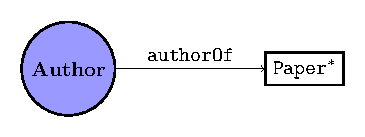
\includegraphics[scale=0.6]{../images/nesting/patterns/00_vertex_pattern.pdf}
				\begin{center}
					Vertex Pattern
				\end{center}
			\end{figure}
		\end{column}
		\hfill
		\begin{column}{.45\textwidth}
			\begin{figure}
				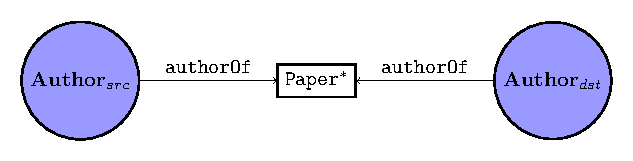
\includegraphics[scale=0.45]{../images/nesting/patterns/00_path_pattern.pdf}
				\begin{center}
					Edge Pattern
				\end{center}
			\end{figure}			
		\end{column}
	\end{columns}
	\begin{center}
		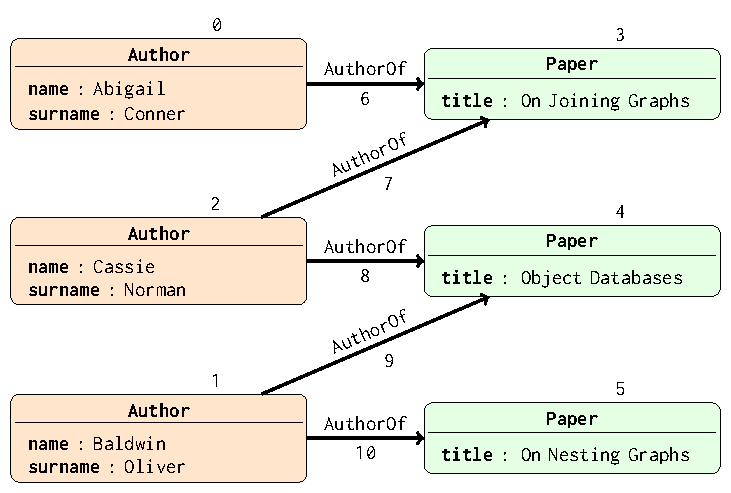
\includegraphics[height=.5\textheight]{../images/nesting/patterns/04bibliography.pdf}\\
		Input Bibliography Network
	\end{center}
\note{In questo problema specifico, imponiamo che 1) esista un sottografo in comune alle due componenti, e 2) che ogni sorgente e destinazione dell'arco possa corrispondere ad un vertice che \`e stato precedentemente annidato.}
\end{lucido}





\begin{lucido}[Desired Result]
\begin{center}
	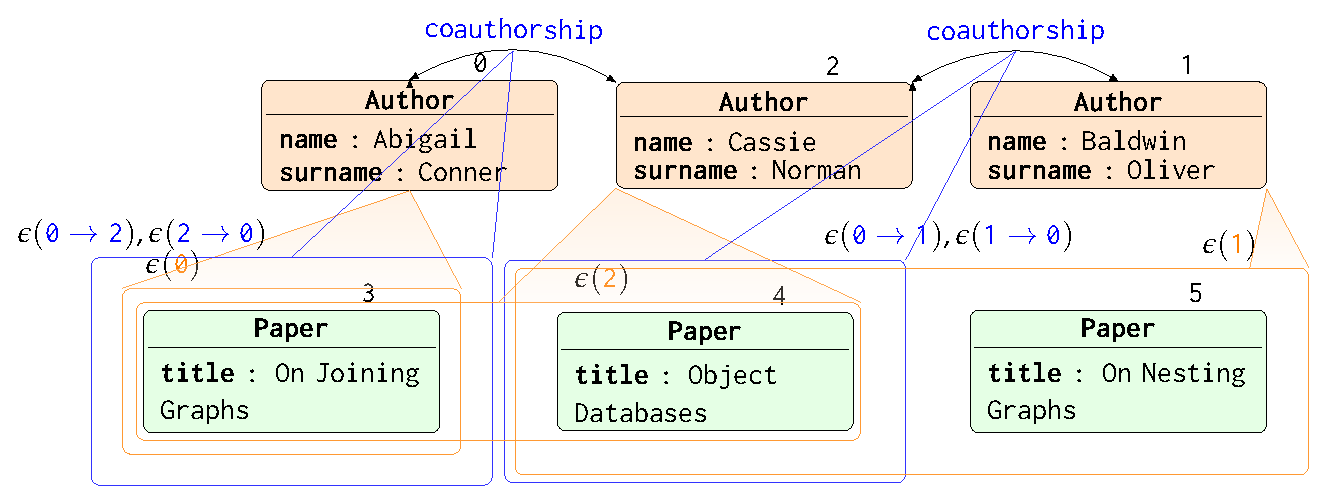
\includegraphics[width=.9\textwidth]{../images/nesting/patterns/042nested.pdf}\\
	Expected result
\end{center}
\end{lucido}

\begin{lucido}[Research Goals]
\begin{enumerate}[<+->]
	\setbeamertemplate{enumerate items}[circle]
	\item As for graph joins, the data model must enhance the \remark{serialization} of both operands and graph result.
	
	\item The logical \remark{graph nesting} operator must be general enough to support both the THoSP algorithm and other graph summarization tasks.
	
	\item Grouping can be avoided by defining a \remark{nesting index}, through which the containment is associated to the container. This can be achieved by extending the Graph Join's data structures with the aforementioned data structure.
	
	%\item The operands' representations model should support property hash joins for backward compatibility.
\end{enumerate}
\end{lucido}

\section{Logical Model}
\begin{multilucido}[Design]
	\begin{sottolucido}
		The nested (property) graph data model is an extension of the logical model for graph joins. Therefore, we want to preserve the same assumptions:
		\begin{itemize}
			\setbeamertemplate{itemize items}[square]
			\item The resulting nested graph is not a materialized view (as in SQL's \texttt{SELECT}).
			\item The nested graph is serialized by only using the ID information. Attribute, values and labels can be completely reconstructed from these informations and the pattern rewriting information.
		\end{itemize}
	\end{sottolucido}

\begin{sottolucido}
	The following modelling choices allow the reconstruction of the required pieces of information:
	\begin{itemize}
		\setbeamertemplate{itemize items}[square]
		\item Vertices and edges are distinctly identified by ids ($\mathbb{N}^2$).
		\item A nested graph database is a property graph, where each vertex and edge may contain (\remark{nest}) another property graph ($\nu, \epsilon$).
		\item Each vertex or edge within the graph can be considered as a possible graph operand.
	\end{itemize}
\end{sottolucido}
\end{multilucido}





\begin{lucido}[Definition]
\hspace*{-3pt}\makebox[\linewidth][c]{\begin{tcolorbox}[width=1.2\textwidth,title=Graph Nesting]
		A nested graph database is a nested graph, where each vertex and edge may represent a graph. Given a nested graph $G=(\mathcal{V},\mathcal{E})$, a vertex pattern $g_V$, a edge pattern $g_E$ vertex pattern containing grouping references: 
		\[\begin{split}
		\alert{\eta_\iota^{\textbf{keep}}(G)}=\Big\langle&\Set{v\in \mathcal{V}|g_V(v)=\emptyset,\textbf{keep}}\cup \iota(g_V(G)),\\	
		&\Set{e\in \mathcal{E}|g_E(e)=\emptyset,\textbf{keep}}\cup \iota(g_E(G))\Big\rangle
		\end{split}\]
		where $\iota$ is an indexing function associating to each matched graph into one new single identifier not appearing in $G$, and keep is set to true whether the non-traversed vertices and edges must be preserved into the final graph. The newly generated nested graph is inserted into the graph database which also contains $G$. Values associated to both nested vertices and edges are determined by user defined functions.
\end{tcolorbox}}
\end{lucido}

%\section{Physical Model}

\section{THoSP Algorithm}
\begin{lucido}[Physical Model]
Motivations:
\begin{enumerate}
	\setbeamertemplate{enumerate items}[circle]
	\item Reduce the number of graph visiting times by visiting the subpattern first, and then extending the visit to the remaining patterns.
	\item Represent the nested graph as an adjacency list enriched with an external nesting index.
\end{enumerate}
The algorithm uses the same principles that were adopted for implementing graph joins:
\begin{itemize}
	\setbeamertemplate{itemize items}[square]
	\item Use memory mapping (OS buffering).
	\item Serialized graphs represent vertices  associated to both ingoing and outgoing edges.
	\item No additional indexing structures are exploited.
\end{itemize}
\end{lucido}

\begin{lucido}[Example]
	\tikzstyle{selected edge} = [draw,line width=5pt,-,green!50]
\tikzset{
	entity/.code={
		\tikzset{
			rounded corners,             
			name=#1,
			inner sep=2pt,
			every entity/.try,
		}%
		\def\entityname{#1}%
	},
	elabel/.style = {
		above,midway,sloped
	},
	eprop/.style = {
		draw=black, text width=2.2cm, below, midway, sloped
	},
	entity anchor/.style={matrix anchor=#1},
	every entity/.style={
		draw,
	},
	every property/.style={
		inner xsep=0.20cm, inner ysep=0.075cm, anchor=west, text width=1.75in
	}
}
\def\property#1{\node[name=\entityname-#1, every property/.try]{\propertysplit#1;};}
\def\properties{\begingroup\catcode`\_=11\relax\processproperties}
\def\processproperties#1{\endgroup%
	\gdef\propertycode{}%
	\foreach \p in {#1}{%
		\expandafter\expandafter\expandafter\gdef\expandafter\expandafter\expandafter\propertycode%
		\expandafter\expandafter\expandafter{\expandafter\propertycode\expandafter\property\expandafter{\p}\\}%
	}%
	\propertycode%
}
\def\propertysplit#1:#2;{\textbf{#1}:#2}

\def\entitynamenode{%
	\node[every entity name/.try] (\entityname-name) {\textbf{\entityname}};
	\draw (\entityname-name.south west) -- (\entityname-name.south east);
	\\[1ex]
}
\tikzset{
	every entity name/.style={every propertred!50y/.try, align=center}
}

\resizebox{\textwidth}{!}{\begin{tikzpicture}[every node/.style={font=\ttfamily\Large}, node distance=0.5in]
	\matrix [entity=Author,fill=orange!20,label={above right:0}]  (a1) {
	\entitynamenode
	\properties{
		name : Abigail,        
		surname : Conner
	}
};
\matrix [entity=Author,fill=orange!20,label={above right:1}] at (0,-6) (a2) {
	\entitynamenode
	\properties{
		name : Baldwin,        
		surname : Oliver
	}
};
\matrix [entity=Author,fill=orange!20,label={above right:2}] at (0,-3) (a3) {
	\entitynamenode
	\properties{
		name : Cassie,        
		surname : Norman
	}
};

\matrix [entity=Paper,fill=green!10,label={above right:3}] at (9,0) (s1) {
	\entitynamenode
	\properties{
		title : On Joining Graphs
	}
};
\matrix [entity=Paper,fill=green!10,label={above right:4}] at (9,-3) (s3) {
	\entitynamenode
	\properties{
		title : Object Databases
	}
};
\matrix [entity=Paper,fill=green!10,label={above right:5}] at (9,-6) (s2) {
	\entitynamenode
	\properties{
		title : On Nesting Graphs
	}
};

\draw[->,very thick] (a1) -- (s1) node [elabel,label={below:6}] {AuthorOf};
\draw[->,very thick] (a3) -- (s1) node [elabel,label={below:7}] {AuthorOf};
\draw[->,very thick] (a3) -- (s3) node [elabel,label={below:8}] {AuthorOf};
\draw[->,very thick] (a2) -- (s3) node [elabel,label={below:9}] {AuthorOf};
\draw[->,very thick] (a2) -- (s2) node [elabel,label={below:10}] {AuthorOf};
\node at (30,-17) {};

\begin{pgfonlayer}{background}
\node<2-5>[inner sep=10pt,rounded corners,fill=green!50,fit=(s1)]{};

\node<3,5>[inner sep=10pt,rounded corners,fill=green!50,fit=(a1)]{};
\draw<3,5>[->,selected edge] (a1) -- (s1) {};

\draw<4-5>[->,selected edge] (a3) -- (s1) {};
\node<4-5>[inner sep=10pt,rounded corners,fill=green!50,fit=(a3)]{};

\node<6-8>[inner sep=10pt,rounded corners,fill=green!50,fit=(s3)]{};
\node<6,8>[inner sep=10pt,rounded corners,fill=green!50,fit=(a3)]{};
\node<7-8>[inner sep=10pt,rounded corners,fill=green!50,fit=(a2)]{};
\draw<6,8>[->,selected edge] (a3) -- (s3) {};
\draw<7-8>[->,selected edge] (a2) -- (s3) {};

\node<9>[inner sep=10pt,rounded corners,fill=green!50,fit=(s2)]{};
\node<9>[inner sep=10pt,rounded corners,fill=green!50,fit=(a2)]{};
\draw<9>[->,selected edge] (a2) -- (s2) {};
\end{pgfonlayer}
	
\matrix<2-> [entity=Paper,fill=green!10,label={above right:3}] at (10,-16) (s1p) {
	\entitynamenode
	\properties{
		title : On Joining Graphs
	}
};
\matrix<6-> [entity=Paper,fill=green!10,label={above right:4}] at (19,-16) (s3p) {
	\entitynamenode
	\properties{
		title : Object Databases
	}
};

\node<8->[inner sep=25pt,rounded corners,draw=blue!80,fit=(s3p),label=above right :{$\epsilon({\color{blue}\texttt{0}\to\texttt{1}}),\epsilon({\color{blue}\texttt{1}\to\texttt{0}})$}] (12cp){
};

\matrix<9-> [entity=Paper,fill=green!10,label={above right:5}] at (26,-16) (s2p) {
	\entitynamenode
	\properties{
		title : On Nesting Graphs
	}
};
\matrix<3-> [entity=Author,fill=orange!20,label={above right:0}] at (11,-10) (a1p) {
	\entitynamenode
	\properties{
		name : Abigail,        
		surname : Conner
	}
};

\node<3->[inner sep=10pt,rounded corners,draw=orange!80,fit=(s1p),
label={above left:$\epsilon(\texttt{\color{orange}0})$}] (s1cp){
};
\draw<3->[color=orange!80] (a1p.south) -- (s1cp.north west);
\draw<3->[color=orange!80] (a1p.south) -- (s1cp.north east);
\path<3->[top color=orange!50, bottom color=orange!10,opacity=0.2] (a1p.south) -- (s1cp.north west) -- (s1cp.north east) -- (a1p.south);

\node<5->[inner sep=25pt,rounded corners,draw=blue!80,fit=(s1p),
label={above:$\epsilon({\color{blue}\texttt{0}\to\texttt{2}}),\epsilon({\color{blue}\texttt{2}\to\texttt{0}})\qquad \qquad\qquad\qquad\qquad $ }
%,label=below :{$\epsilon(\texttt{\color{blue}20})$}
] (02cp){
};


\node<6->[rounded corners,draw=orange!80,fit=(s1p) (s3p),
label={above right:$\epsilon(\texttt{\color{orange}2})$}] (c22p) {
};



\matrix<7-> [entity=Author,fill=orange!20,label={above right:1}] at (26,-10) (a2p) {
	\entitynamenode
	\properties{
		name : Baldwin,        
		surname : Oliver
	}
};
\node<7-8>[inner sep=10pt,rounded corners,draw=orange!80,fit=(s3p),
label={above right:$\epsilon(\texttt{\color{orange}1})$}] (s3pft){
};
\draw<7-8>[color=orange!80] (a2p.south east) -- (s3p.north west);
\draw<7-8>[color=orange!80] (a2p.south east) -- (s3p.north east);
\path<7-8>[top color=orange!50, bottom color=orange!10,opacity=0.2] (a2p.south east) -- (s3p.north west) -- (s3p.north east) -- (a2p.south east);
\matrix<4-> [entity=Author,fill=orange!20,label={above right:2}] at (20,-10) (a3p) {
	\entitynamenode
	\properties{
		name : Cassie,        
		surname : Norman
	}
};
\draw<4-5>[color=orange!80] (a3p.south) -- (s1cp.north west);
\draw<4-5>[color=orange!80] (a3p.south) -- (s1cp.north east);
\path<4-5>[top color=orange!50, bottom color=orange!10,opacity=0.2] (a3p.south) -- (s1cp.north west) -- (s1cp.north east) -- (a3p.south);
\draw<6->[color=orange!80] (a3p.south west) -- (c22p.north);
\draw<6->[color=orange!80] (a3p.south west) -- (c22p.north east);
\path<6->[top color=orange!50, bottom color=orange!10,opacity=0.2] (a3p.south west) -- (c22p.north) -- (c22p.north east) -- (a3p.south west);


\draw<5->[latex-latex] (a1p) edge [bend left] node  [elabel,sloped] (c02p) {\color{blue}coauthorship} (a3p) ;
\draw<5->[color=blue!80] (c02p.south) -- (02cp.north);
\draw<5->[color=blue!80] (c02p.south) -- (02cp.north east);

\draw<8->[latex-latex] (a3p.south) edge [bend right] node [elabel,sloped] (c21p) {\color{blue}coauthorship} (a2p.south) ;
\draw<8->[color=blue!80] (c21p.south) -- (12cp.north);
\draw<8->[color=blue!80] (c21p.south) -- (12cp.north east);



\node<9->[inner sep=20pt,rounded corners,draw=orange!80,fit=(s2p) (s3p),
label={above right:$\qquad\qquad\qquad \epsilon(\texttt{\color{orange}1})$}] (c24p) {
};
\draw<9->[color=orange!80] (a2p.south east) -- ($ (c24p.north east) - (1,0) $);
\draw<9->[color=orange!80] (a2p.south east) -- (c24p.north east);
\path<9->[top color=orange!50, bottom color=orange!10,opacity=0.2] (a2p.south east) -- ($ (c24p.north east) - (1,0) $) -- (c24p.north east) -- (a2p.south east);
	\end{tikzpicture}  }
\end{lucido}

\section{Experimental Evaluation}
\begin{lucido}[Dataset]
	We want to show that the combination of THoSP with the proposed physical data model outperforms the query plans for other query languages (Cypher, SPARQL, SQL, AQL).
	
	We performed our tests on both synthetic and real world data, using  $n=1\div 8$ operands with vertex size $10^n$:
	\begin{itemize}
		\item GMark graph generator.
		\item Random samples of Microsoft Academic Graph.
	\end{itemize} 
	
	Our tests' source code is available at:
	\begin{center}
		\url{https://bitbucket.org/unibogb/graphnestingc/src}
	\end{center}
\end{lucido}

\begin{lucido}[Competing DataBases]
Given that the only graph database using Java was the the worst performing one, we implemented our solution only in C++ The graph nesting operator was implemented in each DB language by redurning ID collections.
	
\begin{itemize}
	\item PostgreSQL was used to evaluate SQL queries. We ran the queries directly in \texttt{psql}.
	\item SPARQL queries were evaluated over Virtuoso. SPARQL queries were send via ODBC (C++).
	\item Cypher queries were evaluated over Neo4J. SPARQL queries were send via the \texttt{execute} method.
	\item AQL queries were evaluated over ArangoDB.  We ran the queries directly in \texttt{arangosh}.
\end{itemize}
\end{lucido}

\begin{lucido}[GMark Benchmark]
\resizebox{\textwidth}{!}{\begin{tabular}{@{}cr|rrrr|r@{}}
		\toprule
			\multicolumn{2}{c}{\textbf{Operands Size}} & \multicolumn{5}{|c}{\textbf{\textsc{Two HOp Separated Pattern} Time (C/C++)} (ms)}  \\
$|V|$  & \#Subgraph  &  {SQL+JSON} & SPARQL & AQL  &  Cypher &{\textbf{THoSP}}  \\
		\midrule
		$10$ & $3$  & 2.10 & 11 & 15.00 & 681.40  & 0.11\\
		$10^2$ & $58$  & 9.68 & 63 & 3.89 &  1,943.98 & 0.14\\
		$10^3$ & $968$  & 17.96 & 63 & 12.34 & {\color{red}$>$3.60$\times 10^6$} & 0.46\\
		$10^4$ & $8,683$  & 69.27 & 364 & 46.74 &  {\color{red}$>$3.60$\times 10^6$} & 4.07\\
		$10^5$ & $88,885$  & 294.23 & 4,153 & 508.87 &  {\color{red}$>$3.60$\times 10^6$} & 43.81 \\
		$10^6$ & $902,020$  & 2,611.48 & 50,341 & 7,212.19 & {\color{red}$>$3.60$\times 10^6$} & 563.02\\
		$10^7$ & $8,991,417$  & 25,666.14 & 672,273 & 922,590.00 & {\color{red}$>$3.60$\times 10^6$} & 8,202.93\\
		$10^8$ & $89,146,891$  & 396,523.88 & {\color{red}$>$3.60$\times 10^6$} & {\color{red}$>$3.60$\times 10^6$} & {\color{red}$>$3.60$\times 10^6$} & 91,834.20\\
		\bottomrule
\end{tabular}}
\end{lucido}

\begin{lucido}[Microsoft Academic Graph Benchmark]
	\resizebox{\textwidth}{!}{\begin{tabular}{@{}cr|rrrr|r@{}}
			\toprule
			\multicolumn{2}{c}{\textbf{Operands Size}} & \multicolumn{5}{|c}{\textbf{\textsc{Two HOp Separated Pattern} Time (C/C++)} (ms)}  \\
			$|V|$  & \#Subgraph  &  {SQL+JSON} & SPARQL & AQL  &  Cypher &{\textbf{THoSP}}  \\
			\midrule
			$10$ & 19  & 1.69$\cdot 10^0$   &  3.4$\cdot 10^1$  & 6.57$\cdot 10^{-1}$  & 2.38$\cdot 10^3$    & \textbf{2.82}$\cdot 10^{-1}$\\
			$10^2$ & 255 & 1.75$\cdot 10^0$  & 3.22$\cdot 10^2$ & 2.51$\cdot 10^0$  & 1.01$\cdot 10^4$    & \textbf{3.46}$\cdot 10^{-1}$\\
			$10^3$ & 23,119  & 4.71$\cdot 10^1$ &  1.22$\cdot 10^3$ & 8.18$\cdot 10^1$  & $>$1H & \textbf{1.39}$\cdot 10^{1}$\\
			$10^4$ & 5,411,205  & 1.53$\cdot 10^4$ &  2.77$\cdot 10^5$ & 2.08$\cdot 10^4$  & $>$1H & \textbf{2.58}$\cdot 10^3$\\
			$10^5$ & 97,079,329  & 1.20$\cdot 10^6$ & $>$1H & {\color{red}OOM$^1$}  & $>$1H & \textbf{1.97}$\cdot 10^5$ \\
			$10^6$ & 241,448,529  & $>$1H &           $>$1H & {\color{red}OOM$^1$}  & $>$1H    & \textbf{6.22}$\cdot 10^5$\\
			$10^7$ & 361,759,509  & {\color{red}OOM$^2$} &      $>$1H & {\color{red}OOM$^1$}  & $>$1H      & \textbf{7.74}$\cdot 10^5$\\
			%$10^8$ & --  & -- & $>$1H & $>$1H & $>$1H & --\\
			\bottomrule
	\end{tabular}}
\end{lucido}
\begin{lucido}[Results]
\begin{itemize}
	\item This further benchmarks shows that all the current data model supporting nested representation do not support query plans allowing for a specific case of (graph) nesting.
	
	\item  The proposed approach extended the secondary memory's property graph representation by adding associations to nested vertices and edges.
	
	\item The serialized data structure provides a graph having an external containment data structure.	
	
	\item This data model achieves \alert{structural aggregation} for graph data, where aggregated data
	may preserve the original vertices and edges.
\end{itemize}
\end{lucido}

\begin{lucido}[Further Results]
\begin{description}
	\item[GROQ:] THoSP can be generalized into a more general algorithm.
	\item[Extending current graph query languages:] The sort-hash join technique allows to answer less-equal predicates.
	\item[Generalized Semistructured Model:] This data structure can be generalized into a broader data representation.
\end{description}
\end{lucido}

\begin{lucido}[Future Work]
\begin{description}
	\item[GROQ:] Further benchmarks have to be carried out over this more general general nesting algorithm.
	\item[General Nesting:] Provide a query plan where either grouping or GROQ are used.
\end{description}
\end{lucido}

\appendix
\section{Backup Slides}
\begin{lucido}[Nested Graph Database]
\hspace*{-3pt}\makebox[\linewidth][c]{\begin{tcolorbox}[width=1.2\textwidth,title=Nested Graph DataBase]
			Given a set $\Sigma^*$ of strings,
		a \textbf{nested (property) graph database} $G$ is a tuple $G=\Braket{\VS, \ES, \lambda,\ell,\omega,\nestF,\prov}$, where:
		\begin{itemize}
			\item $\VS,\ES\in \mathbb{N}^2$ s.t. $\VS\cap \ES=\emptyset$
			\item source and target $\lambda\colon \ES\to \VS^2$.
			\item labelling $\ell:\VS\cup \ES\to \wp(\Sigma^*)$
			\item object mapping $\omega:\VS\cup \ES\to\Omega$
			\item vertices' containment: $\nestF\colon (\VS\cup \ES)\to\wp(\VS)$
			\item edges' containment: $\prov\colon(\VS\cup \ES)\to \wp(\ES)$
		\end{itemize} 
		Each vertex or edge $o\in V\cup E$ induces a \textbf{nested (property) graph} as the following pair:
		\[G_o=\Braket{\nu(o),\Set{e\in\epsilon(o)|\lambda(e)\in (\cup_{n\geq 0}\;{\nu\epsilon}^{(n)}(\{o\}))^2}}\]
\end{tcolorbox}}
\end{lucido}
%

\begin{multilucido}[GCEA]
	\begin{sottolucido}[Experimental Evaluation]
		\begin{itemize}
			\item Through the following experiments we want to prove that :
			\begin{enumerate}
				\item The Physical Model with memory mapping provides better results for GCEA than other low-level graph databases and graph libraries.
				\item GCEA with such Physical Model outperforms the query plans for other query languages (Cypher, SPARQL, SQL). 
			\end{enumerate} 
			\item Tests over one \textit{LiveJournal Graph}, $|V|=4,847,571$ and $|E|=68,993,773$. Enriched with \textit{LDBC Social Network Benchmark protocol}:\url{http://jackbergus.alwaysdata.net/BolognaGraph2016.tar.gz}. 
			\[\theta(u,v)\overset{def}{=}u.Year1 = v.Year2\wedge u.Org1 = v.Org2\]
			\item Tests' source code at \url{https://bitbucket.org/unibogb/databasemappings/}.
		\end{itemize}
	\end{sottolucido}


	\begin{sottolucido}[Experimental Evaluation: Physical Design, 1]
		In our soultion graph operands were stored in secondary memory and accessed through
		memory mapping. The graph join result was written in secondary memory.
		\begin{itemize}
			\item BGL 1.60.0 with \textsc{vec} configuration, graph operands in main memory, default serialization.
			\item SNAP with properties only on vertices, graph operands in main memory, default binary serialization.
			\item Transactions and logging were disabled in Sparksee, graph operands in secondary memory.
		\end{itemize}
		Our Physical Design outperforms other solutions on GCEA algorithm. All such solutions are written in C/C++.
	\end{sottolucido}


	\begin{sottolucido}[Experimental Evaluation: Physical Design, 2a]
		Time results supposing that the operands are either loaded in primary memory or
		memory mapped. 
		\begin{tabular}{r|r|rrr}
			\toprule
			\textbf{Operands Size} & \multicolumn{4}{c}{\textbf{GCEA running time, result creation excluded}}\\
			L=R ($|V|$)  &Proposed  & Boost  & SNAP  & Sparksee  \\
			\midrule
			10 & 0.19\,ms & \textbf{0.09}$\times$ & 0.23$\times$ &  9.42$\times$ \\
			100  & 0.18\,ms & \textbf{0.85}$\times$ & 1.72$\times$ & 24.96$\times$ \\
			1\,000  & \textbf{0.31}\,ms & 5.68$\times$ &14.93$\times$ & 88.42$\times$ \\
			10\,000  & \textbf{1.90}\,ms &11.13$\times$ & 26.83$\times$ & 156.42$\times$ \\
			100\,000  & \textbf{32.31}\,ms & 8.73$\times$ & 19.33$\times$ & 81.05$\times$ \\
			1\,000\,000  &  \textbf{332.60}\,ms & 15.42$\times$ & 33.15$\times$ & 171.54$\times$ \\
			\bottomrule
		\end{tabular}
	\end{sottolucido}

	\begin{sottolucido}[Experimental Evaluation: Physical Design, 2b]
			Time results supposing that the operands are either loaded in primary memory or
		memory mapped. 
		\begin{tabular}{r|r|rrr}
			\toprule
			\textbf{Operands Size} & \multicolumn{4}{c}{\textbf{GCEA result creation time}}\\
			L=R ($|V|$)  &Proposed  & Boost  & SNAP  & Sparksee  \\
			\midrule
			10 & \textbf{0.0010}\,ms & 17.00$\times$ & 36.40$\times$ & 738.33$\times$\\
			100  & \textbf{0.0023}\,ms &  5.39$\times$ & 17.04$\times$ & 290.14$\times$\\
			1\,000  &  \textbf{0.0036}\,ms &  7.72$\times$ & 14.67$\times$ & 215.65$\times$\\
			10\,000  &  \textbf{0.3706}\,ms &  4.60$\times$ &  7.61$\times$ &  15.67$\times$\\
			100\,000  & \textbf{39.3428}\,ms &  4.20$\times$ &  5.80$\times$ &  11.70$\times$\\
			1\,000\,000  &  \textbf{3\,207.8738}\,ms &  5.76$\times$ & 12.29$\times$ &  15.50$\times$\\
			\bottomrule
		\end{tabular}
	\end{sottolucido}

	\begin{sottolucido}[Experimental Evaluation: Physical Design, 2c]
		\begin{tabular}{r|r|rrr}
			\toprule
			\textbf{Operands Size} & \multicolumn{4}{c}{\textbf{Operands Indexing+Storing}}\\
			L=R ($|V|$)  &Proposed  & Boost  & SNAP  & Sparksee  \\
			\midrule
			10 &    0.23\,ms           & \textbf{0.68}$\times$ & 0.98$\times$ &  7.73$\times$\\
			100 &    \textbf{0.50}\,ms  & 1.60$\times$          & 5.22$\times$          & 11.76$\times$\\
			1\,000 &    \textbf{3.38}\,ms  & 1.68$\times$          & 6.94$\times$          & 13.47$\times$\\
			10\,000 &   \textbf{34.26}\,ms  & 1.52$\times$          & 7.25$\times$          & 13.84$\times$\\
			100\,000 &  \textbf{355.96}\,ms  & 1.47$\times$          & 6.27$\times$          & 14.73$\times$\\
			1\,000\,000 & \textbf{3\,518.47}\,ms  & 1.89$\times$          & 6.10$\times$          & 17.79$\times$\\
			\bottomrule
		\end{tabular}
	\end{sottolucido}
\end{multilucido}

\begin{multilucido}[GCLE]
	\begin{sottolucido}[$time_1\leq time_2$, ms running time]
			\begin{tabular}{crrrr}
			\toprule
			\multicolumn{1}{c}{Size}&\multicolumn{1}{c}{Neo4J}&\multicolumn{1}{c}{PostgreSQL}&\multicolumn{1}{c}{Virtuoso}&\multicolumn{1}{c}{\textbf{GLEA C++}}\\
			\midrule
			$10^1$&$ 9,359.86\times$&$  82.61\times$&$   37.58\times$&$    0.15$\\
			$10^2$&$ 2,374.98\times$&$  21.57\times$&$10,308.09\times$&$    1.17$\\
			$10^3$&$28,368.97\times$&$ 191.32\times$&$>3.6\cdot 10^6$ ms&$   10.72$\\
			$10^4$&$>3.6\cdot 10^6$ ms&$1616.22\times$&$>3.6\cdot 10^6$ ms&$   98.50$\\
			$10^5$&$>3.6\cdot 10^6$ ms&$>3.6\cdot 10^6$ ms&$>3.6\cdot 10^6$ ms&$ 1,016.44$\\
			$10^6$&$>3.6\cdot 10^6$ ms&$>3.6\cdot 10^6$ ms&$>3.6\cdot 10^6$ ms&$12,583.89$\\
			\bottomrule
		\end{tabular}
	\end{sottolucido}
\end{multilucido}
\subsection{THoSP Pseudocode}
\begin{frame}[fragile]{THoSP Pseudocode}
	\begin{lstlisting}[mathescape=true,language=pseudi]
nest(Cont, patt, u, S):
for each s in S s.t. patt.doSerialize(s):
     Cont.write(<u,s>)

Input: G, gV, gE 
Cont $\leftarrow$ $\emptyset$ 
NestedGraph $\leftarrow$ $\emptyset$ 

a $\leftarrow$ V $\cap$ E \ ($\gamma_V$ $\cup$ $\gamma_E^{src}$ $\cup$ $\gamma_E^{dst}$);
for each v:vertex in G s.t. a(v):
  for each V(u $\rightarrow^{e}$ v):
    $\textbf{u}$ := dtl(u)$_c$ ; nest(Cont, V, $\textbf{u}$, {u,e,v})
    NGraph(V) $\leftarrow$ NGraph(V) $\cup${$\textbf{u}$}
    for each V(w $\rightarrow^{e'}$ v) s.t. E(u $\rightarrow^{e}$ v${}^{e'}\leftarrow$w)
      $\textbf{w}$ := dtl(w)$_c$ ;
      $\textbf{e'}$ := dtl(u,w)$_c$; 
      nest(Cont, E, $\textbf{e'}$, {u,e,v,e',w})
      NGraph(E) $\leftarrow$ NGraph(E) $\cup${$\textbf{u} \rightarrow^{\textbf{e'}} \textbf{w}$}
	\end{lstlisting}
	
\note{Parlare solo di questi due aspetti: 1) il pattern contiene l'informazione di quale componente devo annidare e quale sarà la componente vertice da restituire 2) l'arco mi fornisce l'informazione di quali sorgenti e destinazioni posso collegare.}
\end{frame}

%\begin{multilucido}[General Semistructured Data Model]
	\begin{sottolucido}
		\begin{columns}[onlytextwidth]
			\begin{column}{.45\textwidth}
				\includegraphics[width=\textwidth]{../fig/04model/01NestedToMatch.pdf}
			\end{column}
			\hfill
			\begin{column}{.45\textwidth}
				\includegraphics[width=\textwidth]{../fig/04model/06schema.pdf}
			\end{column}
		\end{columns}
		A graph represented in both the GSM model (left) and in property graphs (right).
	\end{sottolucido}

	\begin{sottolucido}
		Properties:
		\begin{itemize}
			\item Atoms and collections are represented as objects.
			\item GSM allows property graphs with nested content.
			\item Schema dependency is provided through structural containment.
		\end{itemize}
		Results:
		\begin{itemize}
			\item The proposed data structure overcomes current data structures’ limitations.
			\item GSM allows structural aggregation.
			\item  GSM provides data, model and metamodel pieces of information.
			
		\end{itemize}
	\end{sottolucido}
\end{multilucido}
%\begin{multilucido}[GSQL Operators]
	\begin{sottolucido}
		\centering
		\smartdiagram[constellation diagram]{GSQL Operators, Create, Map, Elect, Disjoint, Fold}
	\end{sottolucido}

	\begin{sottolucido}
		It is possible to define a query language expressing both traversal queries and algebraic operators:
		\begin{description}
			\item[Create] Creates a new object within the GSM database (atoms, objects, collections).
			
			\item[Map] Transforms all the objects within the GSM databas. Allows to express projections, ``select''s and to nest existing elements.
			
			\item[Elect] Elects over which object the n-ary operation has to be performed (Similar to SQL's from).
			
			\item[Disjoint] This operator jointly with map and elect allows to express all the n-ary relational operators. 
			
			\item[Fold] Iteration over an arbitrary \alert{finite} set. Allows iteratively apply the expression's evaluation.  
			
		\end{description}
	\end{sottolucido}
\end{multilucido}

\begin{lucido}[GSQL: Future Works]
\begin{itemize}
	\item Find equivalence rules.
	\item Find optimization by grouping the atomic statements.
\end{itemize}
\end{lucido}

%\begin{multilucido}[Data Integration]
	\begin{sottolucido}
		Schema Oriented, uniform data representation:
		\begin{itemize}
			\item A schema can be always extracted if missing (generalization).
			\item Schema alignment allows to find data similarities.
			\item All the data source schemas shall be aligned to the final hub schema.
		\end{itemize}
	\end{sottolucido}

	\begin{sottolucido}
		Query Oriented (Local/Global as a view):
		\begin{itemize}
			\item The schema alignment can be represented as a query rewriting.
			
			\item We can perform each query separately on the original sources first and then integrate the intermediate results (LAV) or translate and align the data first and then perform the query (GAV).
			
			\item  In both scenarios, part of the query has to be performed on top of the intermediate representation.		
		\end{itemize}
	\end{sottolucido}
\end{multilucido}

